\documentclass[a4paper]{article}
%--------------------------- package
\usepackage[T1]{fontenc}
\usepackage[utf8]{inputenc}
\usepackage{amssymb}
\usepackage{hyperref}
\hypersetup{
    colorlinks=true,
    linkcolor=black,
    filecolor=black,      
    urlcolor=black,
}
\usepackage{booktabs}
\usepackage{ulem}
\usepackage{graphicx}
\usepackage{comment}
\usepackage{minted}
\usepackage{tikz}
%---------------------------
%----------------------------------- theorem
\newtheorem{definition}{Definition}
%-----------------------------------
%-------------------------------------- title and settings
\title{\textbf{Achitectures for big data}
\\[1cm]

\includegraphics[scale=0.12]{images/logo_unimi.png}
\\[1cm]
\large 
    University of Milan\\
    Master's Degree in Computer Science\\
    A.Y. 2022/2023
}
\date{} %hide date
\author{Stefano Vallodoro}
\begin{document}
\maketitle
\newpage
\tableofcontents
\newpage
\setlength{\parindent}{0pt}
\setlength{\parskip}{0.8em}
\setcounter{secnumdepth}{3}
\setcounter{tocdepth}{3}
%--------------------------------------
%------------------------------------ chapters
\section{Architecture}

\paragraph{Software Architecture}
What is Software Architecture? \textit{The way different part of the system connect together}. Is based on sub-system and how this sub-system work together

Can be defined as new types of abstraction that capture the essential
properties of major subsystems and how they interact. Software Architecture is the set of fundamental choices that affect the
structure, quality, and efficiency of a software system. This is important
because it affects the system’s scalability, maintainability, and ability to evolve

\begin{definition}\textbf{Webster's dictionary} The art or practice of designing and building structures and especially habitable ones 
\end{definition}

\begin{definition}
A unifying or coherent form or structure
\end{definition}

Why we call Software Architecture "Architecture"? Inherit a lot of ideas and concepts from building architecture. The most important are: \textit{multiple views}; \textit{architectural style}; \textit{styles and materials}

\paragraph{Multiple views}
Building architecture uses multiple views and different stakeholder linked with different natures and accountability.
\begin{itemize}
    \item \textit{Owner}, does not know how, but knows perfectly \textbf{why}
    \item \textit{Architect}, needs to project and formalize something that fit completely with owner’s needs, the \textbf{what}
    \item \textit{Builder}, needs to design \textbf{how} the what will be built
\end{itemize}
For each stakeholder there’s a specific view. How map the idea in Software Architecture? Each developer have a specific view

\paragraph{Architectural style}
The architectural styles has both the list of the design elements and the formal relationships that allow everyone to use the architecture. We can use architecture style both to constrain the architecture and to coordinate operating
architects. Style embodies those decisions that suffer \textit{erosion} and \textit{drift}.
\begin{itemize}
    \item Erosion means that is not completely clear the reasonal between the architecture so the developer use this not in the proper way
    \item Drift means that the architecture was build for a given reason then reason change overtime and the architecture is not able to follow this evolution
\end{itemize}

\paragraph{Styles and materials}
The material aspects of the design elements provide both aesthetic and engineering bases for an architecture. What could be material inside Software Architecture? Frameworks and technologies, the same function can be obtained
using different sub-systems

\paragraph{Project execution pyramid}
\begin{center}
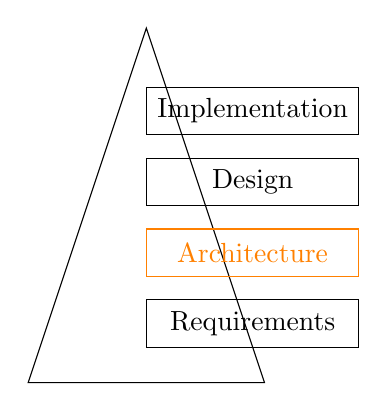
\begin{tikzpicture}[scale=3]
% draw the triangle
\draw (0,0) -- (1.0,0) -- (0.5,1.5) -- cycle;
% draw the rectangles and their labels
\draw (0.5,0.15) rectangle node {Requirements} (1.4,0.35);
\draw[orange] (0.5,0.45) rectangle node {Architecture} (1.4,0.65);
\draw (0.5,0.75) rectangle node {Design} (1.4,0.95);
\draw (0.5,1.05) rectangle node {Implementation} (1.4,1.25);
% add the caption
%\node[above right] at (1.5,1.05) {ciao};
\end{tikzpicture}
\end{center}
It's also described in Perry and Wolf's $1992$ paper, perhaps not as a pyramid shape but as "parts" of the software. We've $4$ layer in the pyramid
    \begin{itemize}
        \item \textit{Requirements}, determination of the information and the characteristics needed by the user of the system
        \item \textit{Architecture}, selection of architectural elements, their interactions and the constraints to satisfy the requirements and serve a basis for the design
        \item \textit{Design}, detailed interfaces of the design elements, algorithms and procedures needed to support the architecture and satisfy the requirements
        \item \textit{Implementation}, representation of the algorithms and data types that satisfy the desing, architecture and requirements
    \end{itemize}

\paragraph{Architecture as a framework for abstractions}
By abstraction we mean identifying a pattern, naming it, defining it, analyzing it and finding a way to invoke it by its name, in order to avoid errors. The basic idea is to omit the right details in the appropriate context, simplifying the interpretation of the result. Example of abstraction are:
\begin{itemize}
    \item \textit{Object Oriented Programming}, abstract data types provide a useful way to organize a software system
    \item \textit{Layered Systems}, OSI layer. System organized hierarchically, with each layer providing service to the layer above it
    \item \textit{Event-oriented programming}, the trigger is the use of this abstraction
\end{itemize}

\paragraph{System-Subsystem Abstraction}
We could use this idea of abstraction to
design system that could be constructed combining subsystem. And this is what an architecture is, a big system that you abstracted combining several subsystem. Each subsystem could be/have an architecture itself and may perform a specific function or a more common function

Identifying and classifying the system functions that are common to many applications is a significant first step to the development of software architecture

%Architecture pillars
\subsection{Architecture pillars}
\begin{enumerate}
    \item \textit{Being the framework for satisfying requirements}, know in advance that all we’re going to build fit completely requirements. Functional, technical and security requirements
    \item \textit{Being the technical basis for design}, modularization and detailed interfaces of the design elements, their algorithms and procedures, and the data types needed to support the architecture and to satisfy the requirements reducing the freedom of the developer
    \item \textit{Being the managerial basis for cost estimation and process management}
    \item \textit{Enabling component reuse}
    \item \textit{Allowing a tidy scalability}, scalability in a people perspective (if I’ve to add some people in the team)
    \item \textit{Avoiding handover and people lock-in}
\end{enumerate}

\begin{definition}
    An architecture is focus on company, mindset, not only technical issue
\end{definition}

%Extra: Foundations for the Study of Software Architecture - Perry, Wolf
\subsection{Extra: Foundations for the Study of Software Architecture - Perry, Wolf}
This paper present a model of software architecture that consists of three components: \textit{elements}, \textit{form}, and \textit{rationale}. Elements are either processing, data, or connecting elements. Form is defined in terms of the properties of, and the relationships among, the elements – that is, the constraints on the elements. The rationale provides the underlying basis for the architecture in terms of the system constraints, which most often derive from the system requirements

\paragraph{Building architecture}
The classical field of architecture provides some of the
more interesting insights for software architecture. While the subject matter for the two is quite different, there are a number of interesting architectural points in building architecture that are suggestive for software architecture: multiple views, architectural styles; style and engineering; style and materials

\paragraph{Context of architecture}
We characterize the different parts of the software
\begin{itemize}
    \item \textit{Requirements}, determination of the information
    \item \textit{Architecture}, selection of architectural elements
    \item \textit{Design}
    \item \textit{Implementation}
\end{itemize}

\paragraph{The model} 
The paper propose the following model of software architecture:
$$\mathit{Software\;Architecture = \{Elements, Form, Rationale\}}$$
In the paper we can distinguish three different classes of architectural elements: processing elements, data elements, connecting elements.

In building architecture, the rationale explicates the underlying philosophical aesthetics that motivate the architect. In software architecture, the rationale instead explicates the satisfaction of the system constraints.

\newpage
\section{Design patterns}
\begin{definition}
Formalization of a best practice to solve a common
problem
\end{definition}

\paragraph{Vendor lock-in}
Vendor lock-in makes a customer dependent on a vendor
for products and services, unable to use another vendor without substantial switching costs. A supplier successfully locks in a customer when:
\begin{itemize}
    \item the cost of changing supplier is higher that the cost of keeping it
    \item without that cost, other suppliers can outperform the actual supplier
\end{itemize}

\paragraph{Knowledge lock-in}
This kind of lock-in happens when the cost of knowledge transfer is higher than the benefit to dismiss a person/team. Again, a Software Architecture can mitigate this risk.
\uline{Avoid the lock-in is the most important challenge for many software architect}.

\paragraph{ETL}
Extract Transform Load involves extracting data from one or more sources, cleaning it up, and then loading it into an output container, which may also have multiple destinations. ETL helps reduce data size and improve quality and consistency by allowing for various transformations. The process can be done all at once or incrementally.

\paragraph{Datalake}
The idea of a Datalake is to have a place to save structured data, obtained from a certain source in unstructured form. On a datalake you only save, you do not delete anything, when a datum changes you insert its modified version. 
    
This approach changes the ETL pattern in ELT, Extract and Load to save to datalake, while at a later time Transforms the data according to the usage. The problem in performing ETL immediately is one in which discarded information is often no longer available

\paragraph{Log Data}
Table that follows a \textit{chrono sequence}, recording events in the order they occur. In these tables past events cannot be undone, they only allow INSERT transactions. Each event is time-stamped. Example: buy/sell transactions of a company.

\paragraph{Registry Data}
A registry data tables describe entities could change over time. There isn’t the idea of chrono sequence, all the
$4$ main verbs (SELECT, INSERT, UPDATE, DELETE ) can be used on it. Example: Bill Of Material 

%Change Data Capture
\subsection{Change Data Capture}
Is a set of design patterns used to determine (and track) the data that has changed.
\begin{itemize}
    \item Eliminates the need for bulk load updating and inconvenient batch windows by enabling incremental loading or real-time streaming of data changes into your target repository
    \item CDC ensures that data in multiple systems stays in sync
\end{itemize}

%Traditional
\subsubsection{Traditional}
\paragraph{Invasive database-side}
\begin{itemize}
    \item \textit{Timestamp on rows}, timestamp of when it happened is added as last update value. The log table only uses this type because there is already a timestamp in the table. The registry needs to add a 'lastUpdate' column, which results in slower insertions and updates
    \item \textit{Version number on rows}, timestamp could be a number. When a change happens, a version $+1$ values is added to the fresh columns. To retrieve the data we need an inner query
    \item \textit{Status indicator}, boolean status. If we have multiple processes we don't know w.r.t. which process is true
    \item \textit{Triggers on table}, a trigger\footnote{Query or code that is executed automatically from the database when a condition happen} is created after any write on the table. They degrade performance for both logs and registries
\end{itemize}

\paragraph{Invasive application-side}
We request that the application perform a replication of every database statement such as \textit{INSERT} or \textit{UPDATE} in a temporary table

\paragraph{Invasive database CPU-side}
\begin{itemize}
    \item \textit{Transaction log scanner}, is technical log of the database itself used for the rollback
    \item \textit{Log shipping}, automatic DB backup
\end{itemize}

%Diff&Where
\subsubsection{Diff\&Where}
Based on the idea that only two kind of data exists: log data; registry data

This pattern is based on
\begin{itemize}
    \item \textit{where-like}, strategy to deal with log like sources. We save the last created value and do the query with that condition
    \begin{minted}
    [
    frame=lines,
    framesep=2mm,
    baselinestretch=1.2,
    bgcolor=white,
    fontsize=\footnotesize,
    linenos
    ]{SQL}
    SELECT * FROM [ TableName ]
    WHERE Timestamp > MAX_TS
    ORDER BY Timestamp
    \end{minted}
    \item \textit{diff-like}, strategy to deal with registry like sources. It’s like the diff on git. 

    I need to make a full table scan, fetch each line one by one comparing with the \textit{KHASH-HASH} list generated in the previous iteration. I need first to save on a sync file the content. To reduce the space I save only hashed values

    This method involves creating a file with tuples consisting of \textit{Khash} and \textit{Hash} values. Hash represents the hash of all columns in each row except for key column, while Khash represents the hash value of key column values. Firstly perform a full table scan and apply the hash function to identify any new rows. A comparison is then made between the current and previous versions of the table (\_old and \_new) to identify any differences.

    \begin{minted}
    [
    frame=lines,
    framesep=2mm,
    baselinestretch=1.2,
    bgcolor=white,
    fontsize=\footnotesize,
    linenos
    ]{python}
    if Khash_old = Khash_new and Hash_old = Hash_new : do nothing
    if Khash_old = Khash_new and Hash_old != Hash_new : update
    if Khash_old not i n Khash_new list : insert
    else : delete
    \end{minted}   
\end{itemize}

%Move and Rename
\subsection{Move and Rename}
\paragraph{Stateless Change Data Capture}
CDC could fail, so you must be able to make a rollback. The idea is to write files in \texttt{.tmp} format to datalake and rename them at the end of the cdc job. On the next iteration, any tmp files, left behind
by any cdc interruption, are deleted. This why the only real atomic operation is the rename
\begin{itemize}
    \item Using temporary filename to automatically tag file just wrote
    \item Renaming every moved file at once at the end of the writing process
    \item A clear final step to be executed at the beginning of any job as an automatic rollback
\end{itemize}

%Adapter
\subsection{Adapter}
We implemented a wrapper that serves as a bridge between our application and external services. This wrapper effectively maps all the interfaces of our external service. As a result, our application is designed to only interact with these services through the interfaces exposed by our wrapper. If in the future we decide to switch to a different Data Lake provider, we can simply update the wrapper to accommodate the new integration without needing to modify the entire application. \uline{This is how you can destroy the vendor lock-in}, real impact on the money for your company

\newpage
\section{MapReduce}
MapReduce is a programming model that was introduced in a Google paper in $2003$ with the aim of accelerating parallel processing of multiple nodes. It works by combining a \textit{map} function, which transforms the input data into key-value pairs, with a \textit{reduce} function, that merges all intermediate values associated with the same intermediate key.

We starting to split using the key, a key is not a unique key, is something you would like to aggregate. A single key is only on a given node. MapReduce works well if you’re able to reduce the communication between the nodes.

Then apply the reduce. It takes couple of rows with the same key and then apply a function to the two value until couple by couple there’re no more couple of lines with the same key

\newpage
\section{Hadoop}
Hadoop is a framework built to facilitate the development of multi-node services. Core idea behind Hadoop is that \textit{hardware can fail}, so Hadoop is a way to enhance reliability on your cluster. Based on three main components:
\begin{enumerate}
    \item \textit{Storage}, HDFS
    \item \textit{Resource management}, YARN
    \item \textit{Parallel computation}, MapReduce
\end{enumerate}

%Hadoop architecture
\subsection{Hadoop architecture}
\begin{itemize}
    \item \textit{Job Tracker}, service that decide where a given task should be executed
    \item \textit{Task Tracker}, accept the task from a Job Tracker. Each task tracker expose the number of slots that represents its capability of run parallel tasks and send an \textit{heartbeats} and \textit{blockreport} to the Job Tracker every minute to reassure it is still alive.
    \item \textit{Name node}, it keeps the directory tree of all files in the file system, and tracks where across the cluster the file data is kept. It's the Single Point of Failure of an Hadoop application.
    \item \textit{Data node}, where data is phisically stored. Each file is stored as a sequence of same sized block, each block is replicated for fault tolerance
\end{itemize}

HDFS has a master/slave architecture. An HDFS cluster consists of a single NameNode, a master server that regulates access to files by clients. In addition, there are a number of DataNodes, usually one per node in the cluster.

Internally, a file is split into one or more blocks and these blocks are stored in a set of DataNodes. The NameNode executes file system namespace operations like opening, closing, and renaming files and directories. The DataNodes are responsible for serving read and write requests from the file system’s clients


%HDFS: Hadoop Distributed File System Storage
\subsection{HDFS: Hadoop Distributed File System Storage}

\paragraph{Simple Coherency Model}
HDFS applications need a write-once-read-many access model for files. A file once created, written, and closed need not be changed except for appends and truncates. Appending the content to the end of the files is supported but cannot be updated at arbitrary point. This assumption simplifies data coherency issues and enables high throughput data access

\paragraph{HDFS policy replication}
Optimizing replica placement distinguishes HDFS from most other distributed file systems improving data reliability, availability, and network bandwidth utilization.

Large HDFS instances run on a cluster of computers that commonly spread across many racks. Communication between two nodes in different racks has to go through switches. The NameNode determines the rack id each DataNode belongs to. In most cases, network bandwidth between machines in the same rack is greater than network bandwidth between machines in different racks

\uline{Rack} is a physical container with internally very high network bandwidth.

\begin{enumerate}
    \item \textit{Replicate the entire rack}, prevents losing data if an entire rack fails but increases the cost of writes because a write need to transfer block to multiple racks
    \item \textit{Two rack factor 3 replication placement}, one replica in a Data Node where the writer task is, another replica in a node in a different remote rack and the last in a different node in the same remote rack. In this way improves the write performance
\end{enumerate}

\paragraph{HDFS reliability} 
Reliability is the capability of the system to have hardware failure without affecting the functionality.

DataNodes are reliable, because NameNode knows perfectly the status of each DataNode. After long time-out NameNode can replicate on a different DataNode. The real weak point are NameNodes. For this reason there’s a possibility of having configuration of HDFS with more than one node using \textit{QJM}

\uline{Quorum Journal Manager} means that are multiple NameNodes with only one in active state and all the other in stand-by state. The QJM ensures that data is available on other nodes, thus maintaining data consistency across the entire cluster. This increases the availability and security of the data, making it an essential component of HDFS.

\newpage
\section{Apache Spark}
Apache Spark allows developers to run multiple tasks in parallel across hundreds of machines in a cluster or across multiple cores on a desktop

 It is based on \textit{in-memory computation}, it saves and loads the data in and from the RAM rather than from the disk, which is a big advantage of Apache Spark over several other big data Frameworks. 

%Apache Spark architecture
\subsection{Apache Spark architecture}
\begin{itemize}
    \item \textit{Master}\\
    It is the only one responsible for negotiating resources with the ResourceManager, based on the resource availability Master schedule tasks. It is created on the same node of driver
    \item \textit{Driver}\\
    Driver is a Java process. This is the process where the $main()$ method of our Scala, Java, Python program runs. It executes the user code and creates a SparkSession or SparkContext and it is responsible to create DataFrame, RDD, execute SQL, perform Transformations and Actions.
    \item \textit{SparkContext}\\
    Core object for Apache Spark, it’s the only way to create Spark specific type. It's a Singleton created by Spark Driver inside Spark Driver JVM. The gateway point of Spark in Apache functionality is the Spark context, it guides how to access the Spark cluster
    \item \textit{Worker}\\
    When a SparkContext is created, each worker starts an executor as a separate process (JVM), and connects back to driver program to receive serialized code
    \item \textit{Executor}\\
    Executor resides in the Worker node. Run an individual task and return the result to the Driver. It can cache (persist) the data in the Worker node
\end{itemize}

\paragraph{Spark is lazy}
Means that Spark compute the result only when it is needed. \uline{The computations happen only when the driver requires a result to be shown}. The transformations are only actually computed when an action is called, this design enables Spark to run more efficiently

\paragraph{How does spark run}
\begin{itemize}
    \item User submits an application using \textit{spark-submit}
    \item The Driver program will be launched inside Application Master
    \item Spark Driver Program will communicate with the Resource Manager
    \item Resource Manager will then allocate containers and Spark Driver Program would start Executors on all the allocated containers and assigns tasks to run
    \item All the Executors will communicate directly with the Spark Driver program and the output from all the executors will be collected by the driver
    \item Once the tasks are finished on each of the executors, the driver program will call $SparkContext.stop()$ method which will terminate the executors and release the underlying resources
\end{itemize}

\paragraph{Basic spark memory management}
\begin{itemize}
    \item Execution memory: used for computations during tasks like sorting, aggregations, and joins
    \item Storage memory: used for caching and circulating data across the cluster
    \item User memory: used to store data required for RDD conversion
    \item Reserved memory: used to reserve space for Spark's internal objects
\end{itemize}
Execution and Storage memory share a unified region in Spark. This means that when no computations are taking place, storage can utilize all available memory, and vice versa.

\paragraph{Spark job}
Each Spark job contains one or more actions, which are split into stages to achieve parallelism. These stages are further split into tasks, which are spread across the executors. Each task handles a subset of the data and can run in parallel.

\paragraph{Transformations and actions}
\begin{itemize}
    \item \textit{Transformations}: Transformations are added to the directed acyclic graph (DAG) and don’t return results until an Action is invoked. A transformations creates a new dataset from an existing one. Some available transformations are \textit{.map()}; \textit{.filter()}; \textit{.join()}; \textit{.reduceByKey()}; \textit{.cartesian()}

    It assumes that the transformations are deterministic and stateless, meaning the output depends only on the input and not on any external state and that the transformations are lazy, meaning they will not be executed until an action is called.
    \item \textit{Actions}: return a value after running a computation on an RDD, is one of the way to send result from Executors to the Driver. Some available action are \textit{.collect()}; \textit{.count()}; \textit{.stats()}
\end{itemize}

\paragraph{Resilient Distributed Database} 
RDD is a highly restricted shared memory model, that is, RDD is a read-only partition record collection, so it cannot be modified. So, we apply an operation and store results in another RDD. 

There are two ways to create RDDs: parallelizing an existing collection in your driver program, or referencing a dataset in an external storage system

Is based on the idea of distributed object. This means, it stores the state of memory as an object across the jobs and the object is sharable between those jobs

\paragraph{Shared variables}
Store small variables and share that all over Spark. When a cluster executor is sent a task by the driver, each node of the cluster receives a copy of shared variables. Spark supports two types of shared variables
\begin{itemize}
    \item \textit{Broadcast}, read-only values once on all nodes. For example, shared dictionary in memory to lookup
    \item \textit{Accumulator}, write-only variables. Allow you to count something in a distributed way.
\end{itemize}

\paragraph{Dataframe} 
Dataframes were introduced with a high-level library called \textit{spark-SQL}. DataFrame is very popular especially because it is user-friendly, easy to use, very expressive (similarly to SQL). Logically, a DataFrame is an immutable set of records organized into named columns. It shares similarities with a table in RDBMS.

DataFrames can be constructed from a wide array of sources such as: structured data files, external databases, or existing RDDs. Similar to RDDs, Dataframes are evaluated lazily


%Natural Language Processing
\subsection{Natural Language Processing}

\paragraph{Bag of word}
Express document in a quantitative way. Mathematical representation of the text, as a vector

\paragraph{Cosine similarity}
Create a metric to compute how similar they are. The distance is computed as the cosine of the angle between two vector. Using cosine you’ve fixed minimum and maximum. The more the cosine similarity is close to $1$ the more two text are similar
    
$$\frac{\sum a_i * b_i}{\sqrt{\sum a^2_i} * \sqrt{\sum b^2_i}}$$

It's just the sum of the frequency of each term in both text divided by the norm of first text times the norm of the second text, where a $=$ given text; i $=$ token

\paragraph{TF-IDF}
Is a measure of originality of a word by comparing the number of times a word appears in a doc with the number of docs the word appears in. The idea behind this behavior is to give more importance to terms that appear in the document but are generally infrequent

$$TF-IDF = TF(t,d) * IDF(t)$$

Where $TF(t,d)$ (Term Frequency) represents the frequency of a word in a document, and is calculated as the number of times a word appears in the document divided by the total number of words in the document.

$IDF(t)$ (Inverse Document Frequency) represents the rarity of the word in the set of documents, and is calculated as the logarithm of the ratio between the total number of documents and the number of documents that contain the word

\newpage
\section{Spark to SQL}

\paragraph{Table index} 
Data structure that increases the read performance of a particular database table, in fact it is not necessary to perform a complete scan but the necessary row is identified immediately, at the cost of additional writes and storage space to maintain it. They can be created using one or more columns from a database table

\paragraph{Creation of an index} 
Using a \textit{B-tree+} for example, the data are only in the leaves. The data is initially sorted, you choose a root and add data to it, when it is full, you add another child root and proceed.

\paragraph{SQL server architecture}
How is a SQL Server organized in a physical way? 2 types of files
\begin{itemize}
    \item \textit{Data files}, a collection of \textit{extents} 8 pages each of size 8 kilobytes (64 kbytes). Within each individual page you have the header, the address of the next page (so as to create a concatenation of pages). Often each page contains blank space so that rows can be inserted faster
    \item \textit{Log files}
\end{itemize}

\paragraph{SQL statement execution}
The query is converted to packets of type \textit{Tabular Data Stream}. These TDS packets need to be converted by the \textit{query parser} into a set of operations to be done, called \textit{query tree}.

The \textit{query executor} executes the query and requests from the access methods the pages that are involved in the query. If we are talking about non-select queries, the \uline{log and lock logic} intervenes
\begin{itemize}
    \item Log manager, is the one who is responsible for keeping track of all the updates completed in the system through the transaction logs
    \item Lock manager, during the transaction, the data is in the lock state. It guarantees Consistency and Isolation
\end{itemize}

\paragraph{How to write}
There are three methods for connecting to a database
\begin{itemize}
    \item \textit{Direct connection}, you open a connection with a socket
    \item \textit{Connection pooling}, connections are kept open and are assigned to clients who request them
    \item \textit{Pool fragmentation}, each client has its own pool
\end{itemize}
In Apache Spark, writing a million rows to a database using a direct connection can result in multiple connections being opened for one worker. If we use a connection pool to send data from the worker to the database, the database can be overloaded and become unresponsive due to keeping the ports busy. Having one database and many workers is not an ideal situation in either case.

To solve the problem of multiple workers writing to SQL, one can write all the information to a Data Lake and then write it in bulk to SQL. The idea is to take advantage of the \textit{BCP}, bulk copy program, to copy all new rows from datalake to SQL, and use MERGE to join them to the old table

\newpage
\section{Delta lake}
Delta Lake aims to ensure ACID properties on HDFS, therefore on distributed storage.

\paragraph{Transaction} 
Sequence of operations satisfying ACID properties

\paragraph{ACID properties} 
Properties that are necessary to ensure transactionality
\begin{itemize}
    \item \textit{Atomicity}, each operation of a transaction is atomic
    \item \textit{Consistency}, a transaction must maintain the consistency of the system
    \item \textit{Isolation}, concurrent executions lead to the same result as sequential executions
    \item \textit{Durability}, a transaction cannot be restored after a commit
\end{itemize}

\paragraph{Transacion logs} History of the operations performed by a database, can be useful for rollbacks in cases where some transactions have failed

\paragraph{Log shipping} Logs can be sent to a server to replicate the state of the database and have an exact copy of the system

\paragraph{Delta Lake features}
\begin{itemize}
    \item \textit{Time travel}, possibility of returning the storage state to a specific time snapshot
    \item \textit{UPSERT, DELETE and MERGE}
    \item \textit{Efficient streaming}, information is written quickly since it is divided into small blocks. Blocks are joined together later to speed up readings
    \item \textit{Caching}, cluster nodes can cache information
\end{itemize}

\newpage
\section{SOA: Service Oriented Architecture}
The basis of SOA is to bridge the IT and business worlds

\paragraph{IBM definition}
SOA is an architectural style for creating an enterprise IT ar-
chitecture that leverages the principles of service orientation to achieve a closer
relationship between the business and the information systems that support it.
The \textit{SOA stack} is envisioned as an architecture with 5 layers
\begin{enumerate}
    \item \textit{Operating systems}
    \item \textit{Service components}
    \item \textit{Services}
    \item \textit{Business processes}
    \item \textit{Clients}
\end{enumerate}

\paragraph{Service} 
A service is a resource identified by a name that performs a repetitive business task with a specified outcome. Each service consists of:
\begin{itemize}
    \item Name
    \item Version
    \item Execution type: asynchronous, synchronous
    \item Logging method: before, after
    \item Message in: configuration of incoming messages
    \item Message out: configuration of outgoing messages
    \item Visibility
\end{itemize}

\paragraph{Server catalog} 
Catalog of all available services

\paragraph{Service queue} 
List of service executions

\newpage
\section{From big data to big money}
When architecting an IT solution, two fundamental aspects must be taken into account, \textit{benefit} and \textit{cost}.

%Cost
\subsection{Cost}

\paragraph{Capex}
\textit{Capital expenditure}, encloses funds spent on improving the company's assets, such as buildings, vehicles, machinery or software

\paragraph{Opex}
\textit{Operating expense} refers to the money spent on maintaining the effective functioning of a product or service, such as software license fees

\begin{center}
    \begin{tabular}{lcc} 
    \toprule
        EG & CAPEX & OPEX \\
    \midrule
        Buying software & X &  \\ 
        Buying hardware & X &  \\
        Software ad-hoc solution  & X &  \\
        Monthly software fee &   & X \\
        Cloud service &   & X \\
        Interview consultant for start-ups &   & X \\
    \bottomrule
   \end{tabular}
\end{center}

\paragraph{As a service}
$X$ as a service refers to something offered as a service, the complexity of which is hidden from the end customer. Some examples are:
\begin{itemize}
    \item \textit{Infrastructure as a service}: hardware offered by a certain provider
    \item \textit{Software as a service}: ability to use software without installing it
    \item \textit{Platform as a service}: ability to use complex platforms without worrying about complex configurations
\end{itemize}

%Team development
\subsection{Team development}
\paragraph{Project management} 
Process of bringing a team's work toward the completion of a certain goal by completing all requirements in a given period of time. Achieve all project goals given the constraints

\paragraph{GANTT chart} 
Graph with tasks and weeks, with their associations. Using this chart we can define \textit{how much} because uses a time plan so it's possible calculate the cost.

\paragraph{Waterfall} 
Development method where project phases are sequential, only once one part is finished can the next part begin. It is not flexible, you cannot change requirements in progress

The main problem of waterfall methodologies is assuming predictability. Software development is unpredictable and investing too much time upfront on a plan will inevitably generate waste

\paragraph{Agile} 
You divide the work into sprints, at each sprint the developers deliver a working version of the system.
High-level requirements, formalized in a \textit{Product Backlog}, are gathered before starting. There are several roles:
\begin{itemize}
    \item \textit{Product owner}: takes care of adding Product Backlog priorities. Each requirement in the Product Backlog becomes a \textit{User Story}, each sprint deals with completing a certain amount of it
    \item \textit{Scrum master}: takes care of checking that you don't break/follow the Agile model
    \item \textit{Team}: group of developers
    \item \textit{Stakeholders}: they evaluate the product
\end{itemize}

\newpage
%------------------------------------


\end{document}
